\chapter{Networks from Distances}

So far we have been using existing network graphs. But we can also generate a graph from regular tabular data. Let us take the \emph{iris} data set. For now, we only have flowers as rows and their characteristics as columns. So how do we transform this to nodes and edges?

By looking at similarities. Rows will be nodes and the edge will be created between two rows if their similarity is above a certain threshold. Nice, isn't it?

\begin{figure}[h]
    \centering
    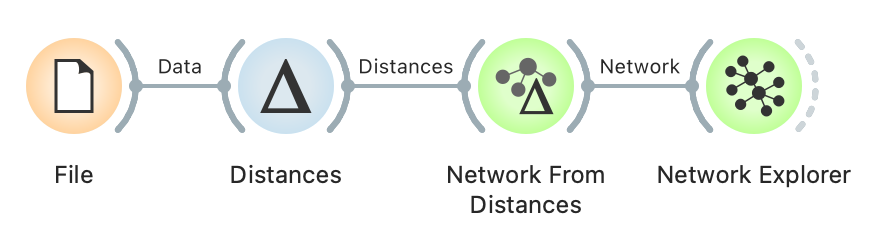
\includegraphics[width=\linewidth]{workflow.png}
    \caption{$\;$}
\end{figure}

First, we need distance matrix, which we can compute with the \widget{Distances} widget. Let's stick with Euclidean distances as it works well with this 4-dimensional data set.

Then pass the distance matrix to \widget{Network from Distances}. The widget enables setting the distances threshold, which we will set to 2.0 percentiles (meaning we keep the top 2\% of the edges that connect the most similar nodes).

\begin{figure}[h]
    \centering
    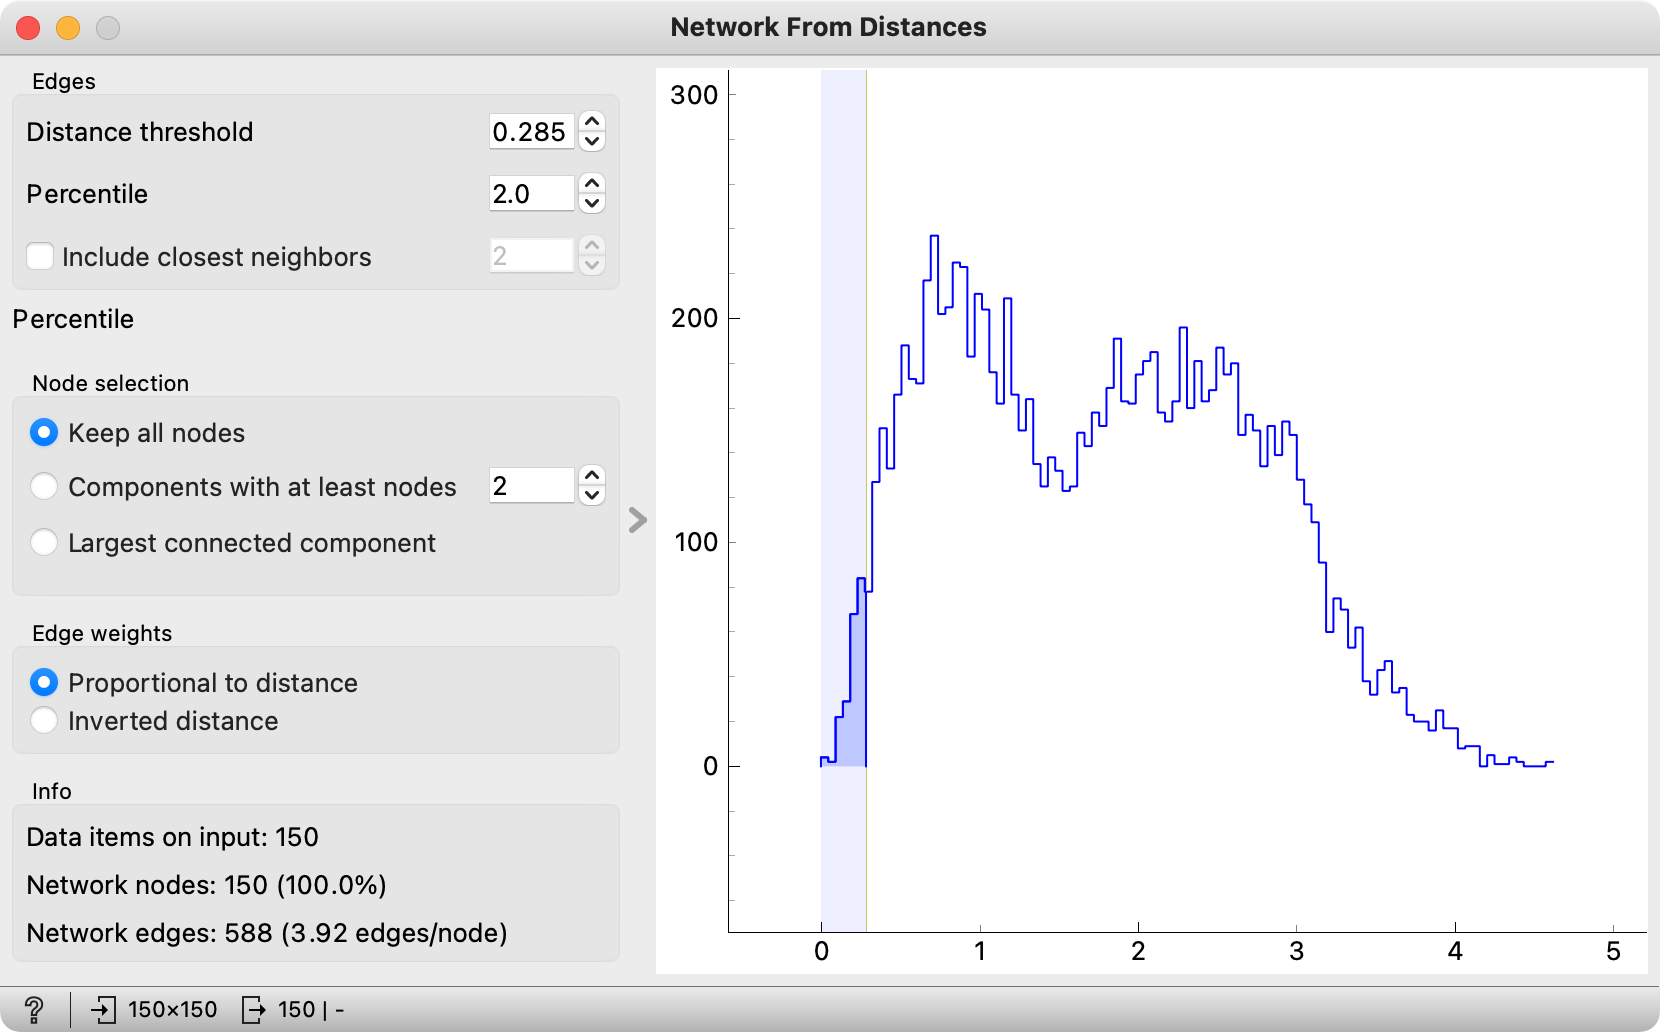
\includegraphics[scale=0.45]{net-from-distances.png}
    \caption{$\;$}
\end{figure}

\newpage

Finally, pass the constructed graph to \widget{Network Explorer}. Remember, this is not a scatter plot. The position of the points is not mapped to any sort of attribute. In the graph, you can simply see which elements are most similar to one another.

\begin{figure*}[h]
    \centering
    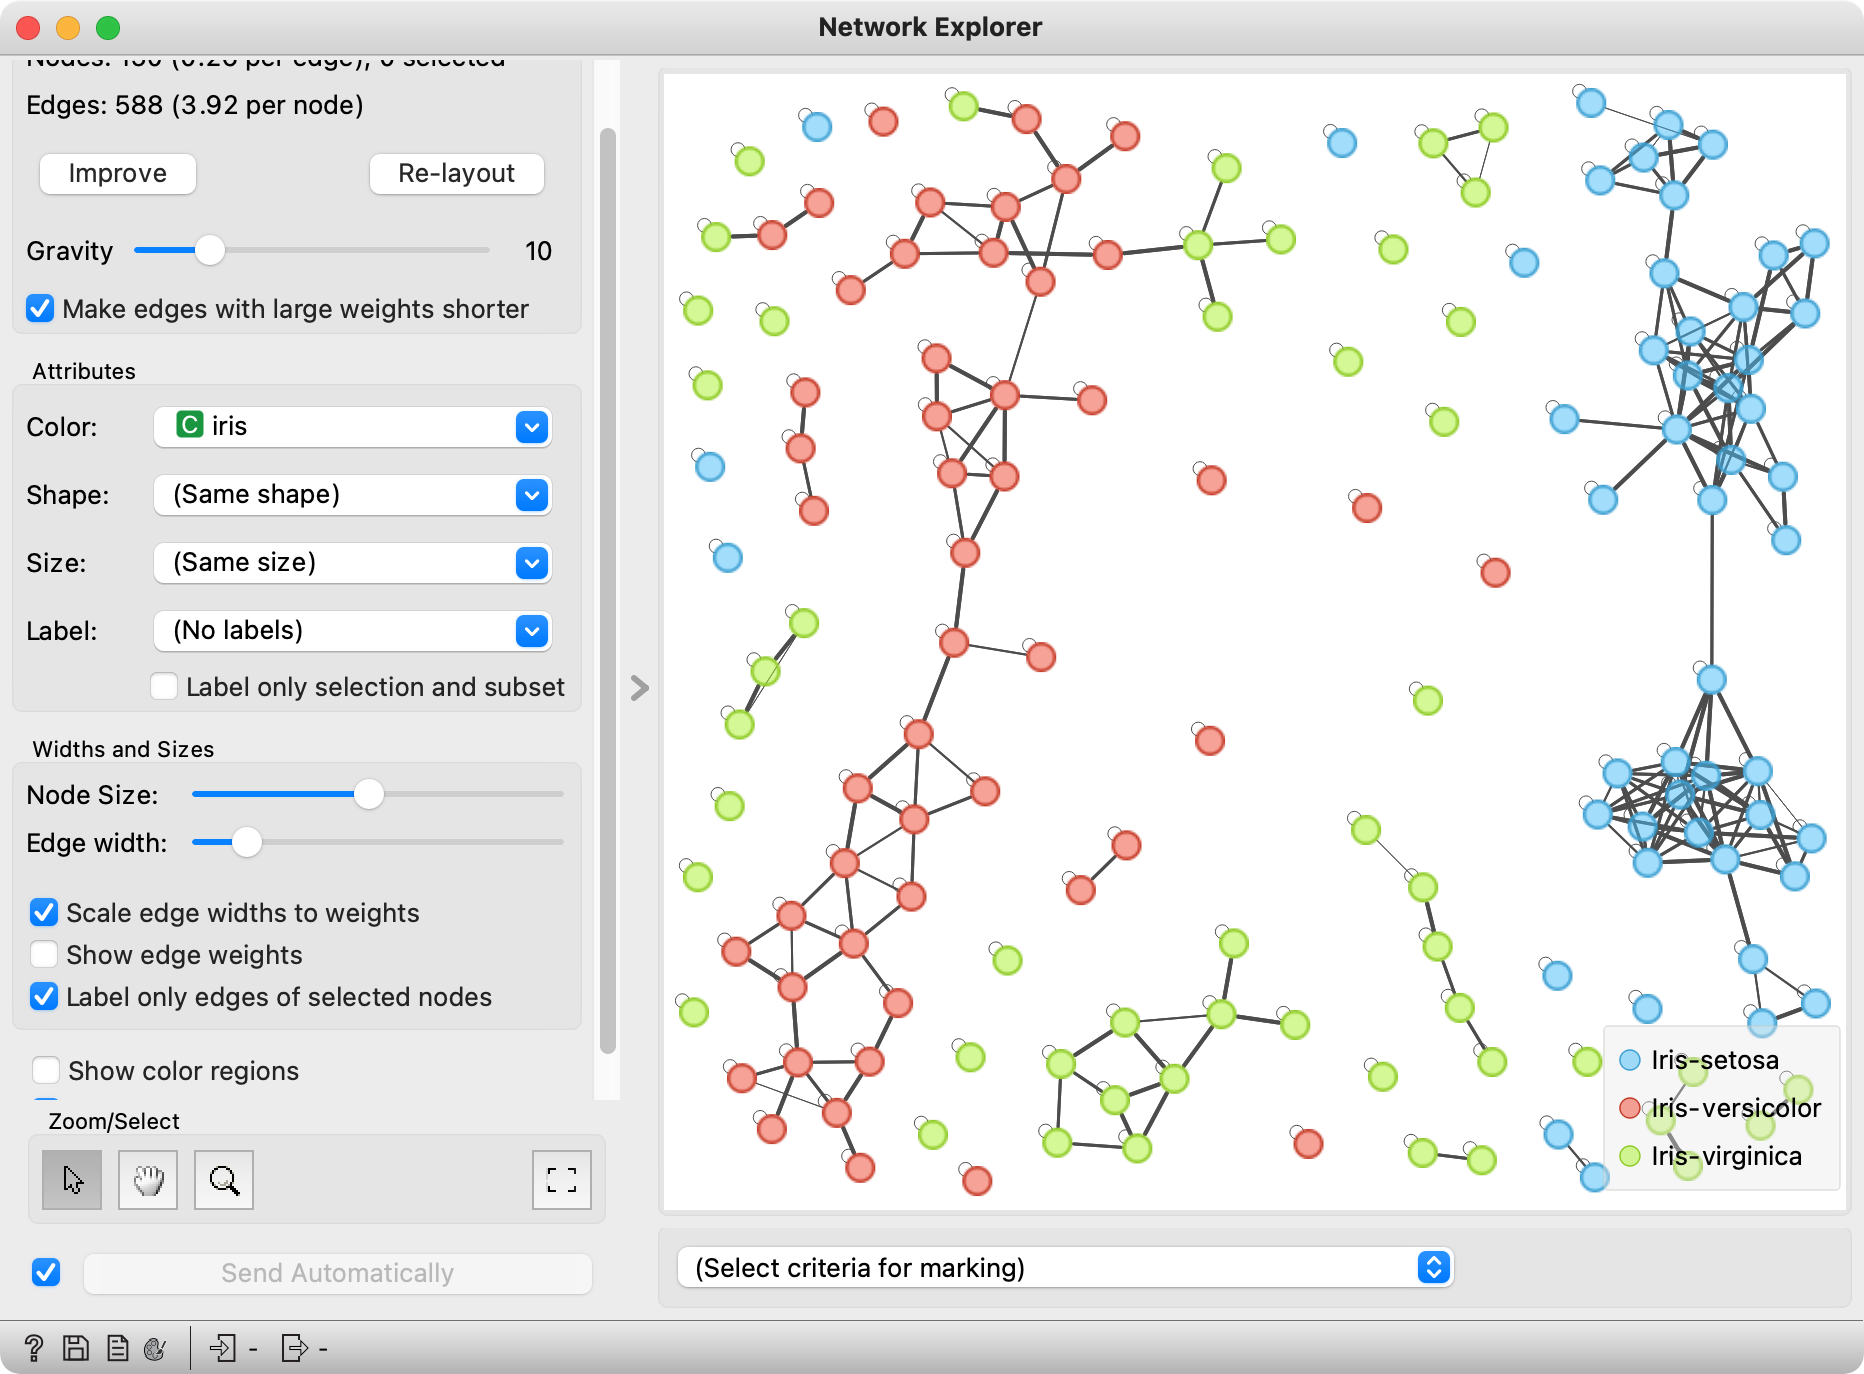
\includegraphics[width=\linewidth]{network-explorer.png}
    \caption{$\;$}
\end{figure*}
